\documentclass[11pt]{article}
\usepackage{geometry,marginnote} % Pour passer au format A4
\geometry{hmargin=1cm, vmargin=1cm} % 

% Page et encodage
\usepackage[T1]{fontenc} % Use 8-bit encoding that has 256 glyphs
\usepackage[english,french]{babel} % Français et anglais
\usepackage[utf8]{inputenc} 

\usepackage{lmodern,numprint}
\setlength\parindent{0pt}

% Graphiques
\usepackage{graphicx,float,grffile,units}
\usepackage{tikz,pst-eucl,pst-plot,pstricks,pst-node,pstricks-add,pst-fun,pgfplots} 

% Maths et divers
\usepackage{amsmath,amsfonts,amssymb,amsthm,verbatim}
\usepackage{multicol,enumitem,url,eurosym,gensymb,tabularx}

\DeclareUnicodeCharacter{20AC}{\euro}



% Sections
\usepackage{sectsty} % Allows customizing section commands
\allsectionsfont{\centering \normalfont\scshape}

% Tête et pied de page
\usepackage{fancyhdr} \pagestyle{fancyplain} \fancyhead{} \fancyfoot{}

\renewcommand{\headrulewidth}{0pt} % Remove header underlines
\renewcommand{\footrulewidth}{0pt} % Remove footer underlines

\newcommand{\horrule}[1]{\rule{\linewidth}{#1}} % Create horizontal rule command with 1 argument of height

\newcommand{\Pointilles}[1][3]{%
  \multido{}{#1}{\makebox[\linewidth]{\dotfill}\\[\parskip]
}}

\newtheorem{Definition}{Définition}

\usepackage{siunitx}
\sisetup{
    detect-all,
    output-decimal-marker={,},
    group-minimum-digits = 3,
    group-separator={~},
    number-unit-separator={~},
    inter-unit-product={~}
}

\setlength{\columnseprule}{1pt}

\begin{document}

\textbf{Nom, Prénom :} \hspace{8cm} \textbf{Classe :} \hspace{3cm} \textbf{Date :}\\
\vspace{-0.8cm}
\begin{center}
  \textit{Je n'aime pas le travail, nul ne l'aime ; mais j'aime ce qui est dans le travail l'occasion de se découvrir soi-même.}  - \textbf{Joseph Conrad}
\end{center}
\vspace{-0.8cm}

\subsection*{Exercice 1 - Calculer}

\begin{multicols}{3}\noindent
    \begin{enumerate}
      \item $5 + \ldots\ldots = 9$
      \item $9 \times 6 = \ldots\ldots$
      \item $2 \div 1 = \ldots\ldots$
      \item $11 - \ldots\ldots = 1$
      \item $\ldots\ldots \div 9 = 3$
      \item $6 \div \ldots\ldots = 2$
      \item $1 \times 10 = \ldots\ldots$
      \item $30 \div 5 = \ldots\ldots$
      \item $15 \div 5 = \ldots\ldots$
      \item $16 - \ldots\ldots = 6$
      \item $9 \times \ldots\ldots = 36$
      \item $10 + \ldots\ldots = 17$
      \item $8 + \ldots\ldots = 16$
      \item $\ldots\ldots + 9 = 19$
      \item $18 - \ldots\ldots = 8$
      \item $\ldots\ldots - 6 = 7$
      \item $\ldots\ldots - 1 = 8$
      \item $8 + 8 = \ldots\ldots$
      \item $\ldots\ldots \times 7 = 7$
      \item $\ldots\ldots \times 10 = 80$
    \end{enumerate}
  \end{multicols}

\subsection*{Problème}

J'aide mon père à faire les courses. Je récupère le ticket de caisse avec les calculs.
\begin{itemize}
  \item $3 \times 2.65 = 7.95$
  \item $2 \times 3.42 = 6.84$
  \item $1.65 \times 2.4 = 3.96$
  \item $6.84 + 3.96 + 1.17 = 19.92$
  \item $20 - 19.92 = 0.08$
\end{itemize}

\textbf{Complète le texte : }

Mon père a acheté deux paquets de Prince à \ldots\ldots\ldots l'un, 1,650 kg de pommes à \ldots\ldots\ldots le kg, \ldots\ldots\ldots packs de bouteilles d'eau à 2,65\euro le pack et une tablette de chocolat à \ldots\ldots\ldots . Il paie avec un billet de \ldots\ldots\ldots . On lui rend \ldots\ldots\ldots centimes.

\subsection*{Sudoku 4x4}

\begin{figure}[H]
  \centering
  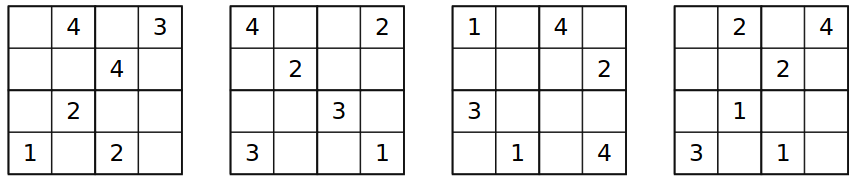
\includegraphics[width=0.8\linewidth]{5x1-calculs/sudoku-4a.png}
\end{figure}

\newpage

\subsection*{Exercice 2 - Calculer}
\textit{en écrivant les étapes et en respectant les priorités de calcul}

\begin{multicols}{3}\noindent

  \begin{enumerate}
    \item $A = 12 \times (7-5)$ 
    \item $B = 10 + (8 - 7)$ 
    \item $C = 11 - 8 + 12 \div 3 \times 7$ 
    \item $D = 2 \times (4+10) + 10 \div (12-7)$ 
    \item $E = 2 + 9 \times 5 \div (3-2)$ 
    \item $F = 8 + 4 \times 10\div (10-(2+6))$ 
  \end{enumerate}

\end{multicols}

\Pointilles[47]

\newpage


\textbf{Nom, Prénom :} \hspace{8cm} \textbf{Classe :} \hspace{3cm} \textbf{Date :}\\
\vspace{-0.8cm}
\begin{center}
  \textit{Je n'aime pas le travail, nul ne l'aime ; mais j'aime ce qui est dans le travail l'occasion de se découvrir soi-même.}  - \textbf{Joseph Conrad}
\end{center}
\vspace{-0.8cm}

\subsection*{Exercice 1 - Calculer}

\begin{multicols}{3}\noindent
    \begin{enumerate}
      \item $\ldots\ldots + 3 = 10$
      \item $4 \times 5 = \ldots\ldots$
      \item $6 \times 2 = \ldots\ldots$
      \item $17 - 7 = \ldots\ldots$
      \item $\ldots\ldots \times 5 = 50$
      \item $\ldots\ldots + 8 = 14$
      \item $7 + 10 = \ldots\ldots$
      \item $4 \times 6 = \ldots\ldots$
      \item $\ldots\ldots \div 7 = 10$
      \item $21 \div \ldots\ldots = 7$
      \item $8 - 5 = \ldots\ldots$
      \item $10 + 2 = \ldots\ldots$
      \item $\ldots\ldots + 4 = 14$
      \item $8 - \ldots\ldots = 7$
      \item $40 \div 8 = \ldots\ldots$
      \item $20 - 10 = \ldots\ldots$
      \item $\ldots\ldots - 10 = 7$
      \item $1 \times 2 = \ldots\ldots$
      \item $30 \div \ldots\ldots = 10$
      \item $10 \div 1 = \ldots\ldots$
    \end{enumerate}
  \end{multicols}

\subsection*{Problème}

J'aide mon père à faire les courses. Je récupère le ticket de caisse avec les calculs.
\begin{itemize}
  \item $3 \times 2.65 = 7.95$
  \item $2 \times 3.42 = 6.84$
  \item $1.65 \times 2.4 = 3.96$
  \item $6.84 + 3.96 + 1.17 = 19.92$
  \item $20 - 19.92 = 0.08$
\end{itemize}

\textbf{Complète le texte : }

Mon père a acheté deux paquets de Prince à \ldots\ldots\ldots l'un, 1,650 kg de pommes à \ldots\ldots\ldots le kg, \ldots\ldots\ldots packs de bouteilles d'eau à 2,65\euro le pack et une tablette de chocolat à \ldots\ldots\ldots . Il paie avec un billet de \ldots\ldots\ldots . On lui rend \ldots\ldots\ldots centimes.

\subsection*{Sudoku 4x4}

\begin{figure}[H]
  \centering
  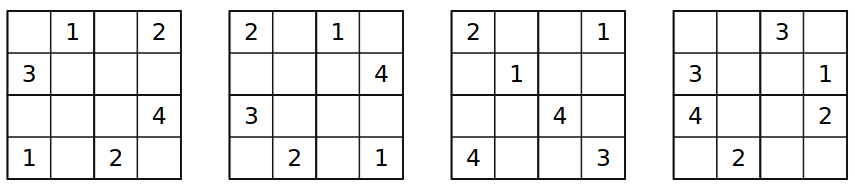
\includegraphics[width=0.8\linewidth]{5x1-calculs/sudoku-4b.png}
\end{figure}

\newpage

\subsection*{Exercice 2 - Calculer}
\textit{en écrivant les étapes et en respectant les priorités de calcul}

\begin{multicols}{3}\noindent

  \begin{enumerate}
    \item $A = 40 \times (4 + 5)$ 
    \item $B = 50 - (8 + 12)$ 
    \item $C = 10 \times 8 + 12 \div 3 \times 5$ 
    \item $D = 2 \times (14 - 10) + 20 \div (12-7)$ 
    \item $E = 2 + 9 \times 5 \div (5-4)$ 
    \item $F = 18 + 3 \times 10 \div (10-(5+3))$ 
  \end{enumerate}

\end{multicols}

\Pointilles[47]

\end{document}